\section{问题二求解与分析}
\label{sec:q2}
\subsection{问题的描述与分析}
第二问延续第~\ref{sec:q1} 章的完整方案 $x=(\mathcal P,a,\boldsymbol\pi)$、总体任务执行时间 $C_q$ 和额外 COPY 字节 $D_q$，但重新界定执行任务：一个核心上的全部子图共同构成一个 Task。子图划分与核内顺序仍规定算子的归核、局部先后与跨核边界；改变的是同核子图之间的状态能否延续，以及跨核交接的就绪条件。同一张量若由本核的后续子图使用，可以继续占据 L1 或 UB，从而减少边界写回与重读。驻留时间延长也可能触发自动换出，形成搬运节省与容量压力之间的权衡。

图~\ref{fig:q2_overview} 给出本问的求解脉络。算法按核心级 Task 重建交接与内存生命周期，围绕跨核通信、驻留峰值和并行度提出候选，并沿用完整评价与字典序接受准则。结果分析同时观察五核加速比、与第一问的逐图周期比、额外 COPY 变化和候选来源记录。前两问各自独立寻优，逐图比较反映执行规则与方案选择共同作用后的表现。
\begin{figure}[htbp]
\centering
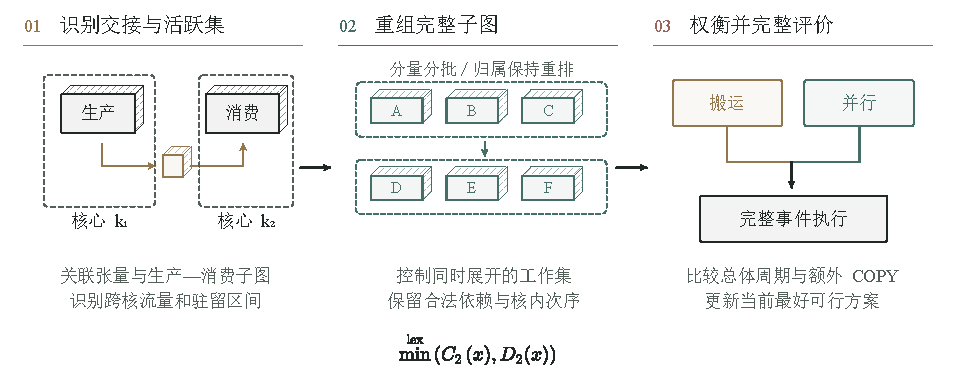
\includegraphics[width=\textwidth]{../求解/问题二/图片/q2_overview.pdf}
\caption{问题二的联合建模与迭代改进框架}\label{fig:q2_overview}
\end{figure}


\subsection{核心级任务的执行模型}
\subsubsection{同核驻留与跨核交接}
对核心 $k$，令 $\pi_k=(i_1,\ldots,i_{m_k})$，其全部子图属于同一 Task，任务标识为 $k$。同核相邻子图按方案顺序执行，但任务边界不在两者之间重复建立。若张量 $t$ 的生产者和后续消费者均位于 $k$，且执行过程未将相应缓冲换出，则消费者可读取本核驻留实例。图~\ref{fig:q2_task} 表示两类路径：同核复用沿着驻留状态传播，跨核依赖则先完成输出搬运，再进入目标核的读入队列。
\begin{figure}[htbp]\centering
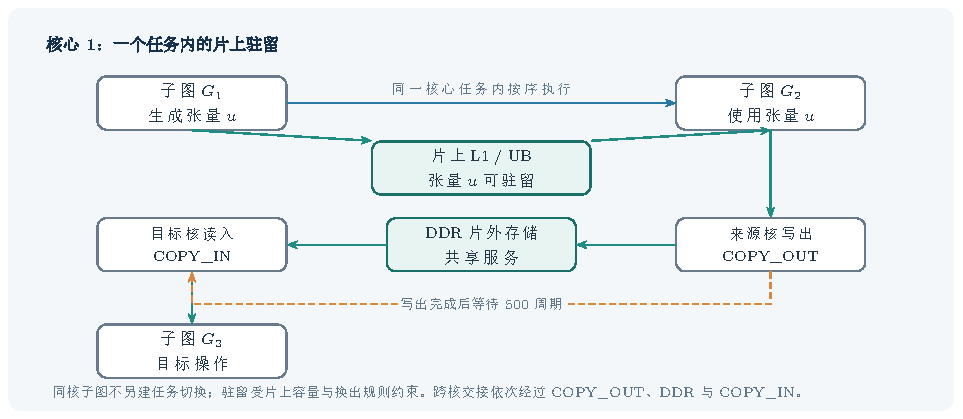
\includegraphics[width=\textwidth]{../求解/问题二/图片/q2_task.pdf}
\caption{核心级 Task 中的驻留与跨核交接}\label{fig:q2_task}
\end{figure}

对于跨核张量 $t$ 的一条交接，设相应 $\mathrm{COPY\_OUT}$ 完成于 $f_t^{\mathrm{out}}$，目标核的 $\mathrm{COPY\_IN}$ 开始于 $s_t^{\mathrm{in}}$。题设要求
\begin{equation}
 s_t^{\mathrm{in}}\ge f_t^{\mathrm{out}}+500.
 \label{eq:q2_handoff}
\end{equation}
若目标操作依赖多个跨核输入，则各输入分别满足式~\eqref{eq:q2_handoff}，其可启动时刻受最晚到达者约束。同核路径直接延续本核任务的存储状态。式~\eqref{eq:q2_handoff} 只是释放读入的必要条件：$\mathrm{COPY\_OUT}$ 和 $\mathrm{COPY\_IN}$ 本身占用共享 DDR，目标核读入流水线、缓冲容量及其他依赖还可能继续推迟完成时刻。

本问保持联合决策变量不变，采用核心级任务的执行映射 $\mathcal E_2$，优化问题为
\begin{equation}
 \min_{x\in\mathcal F_2}^{\mathrm{lex}}\bigl(C_2(x),D_2(x)\bigr).
 \label{eq:q2_problem}
\end{equation}
这里 $\mathcal F_2$ 仍由无环、容量和完整执行可行性共同确定。两问分别重建 COPY、缓冲生命周期和任务就绪时间，再由全局事件执行得到周期。

\subsubsection{活跃集、自动换出与共享带宽}
同核跨子图驻留扩大了复用机会，也延长了活跃区间。实际占用按式~\eqref{eq:capacity} 的缓冲实例集合 $\mathcal B_{k,r}(\tau)$ 检查。部分候选在来源内排序时采用换出前存储需求估计：将核心 $k$ 的子图按 $\pi_k$ 连接，组内按原图拓扑位置排列，得到算子序列。对序列中的张量，其估计生命期从首次生产位置开始；没有本核生产者时从首次使用位置开始，并延续至最后生产或使用位置。记位置 $h$ 上仍处于这一闭区间、归入存储区 $r$ 的张量集合为 $\widehat{\mathcal L}_{k,r}(h;x)$。原位置为DDR的张量在代理中按UB计，同一张量在各核分别计量。定义峰值估计
\begin{equation}
 \widehat M_r(x)=\max_{k,h}\sum_{t\in\widehat{\mathcal L}_{k,r}(h;x)}b_t,
 \qquad r\in\{\mathrm{L1},\mathrm{UB}\}.
 \label{eq:q2_livepeak}
\end{equation}
式~\eqref{eq:q2_livepeak} 估计了自动换出前的逻辑活跃需求，可用于定位候选的驻留压力。完整执行随后依据固定顺序、下一次使用位置和换出资格插入Spill/Retrieve，并按实际缓冲实例检查容量。联合调度与张量置换研究揭示了驻留状态与片外访问的耦合\cite{A16}；内存感知调度研究则讨论了拓扑顺序对活跃集合和峰值存储的影响\cite{A17}。本文将这些分析用于子图划分、归核和核内顺序的候选设计。

额外 COPY 字节 $D_2(x)$ 汇总重建边界搬运及自动换出等题设规定的计量项。搬运字节与执行时间之间还受到事件时序影响。若多个核心同时提交 DDR 请求，第~\ref{sec:q1} 章式~\eqref{eq:bandwidth} 的共享服务率取决于当时在途请求数。局部减少字节，可能因为请求从非关键段移至关键段而并未缩短总体任务执行时间；反过来，适度增加搬运，也可能提前释放依赖或让计算与通信重叠。因此，跨核 COPY 数、驻留峰值和计算负载在候选阶段用于解释与排序，最终保留仍由完整执行的 $(C_2,D_2)$ 判定。

\subsection{面向驻留与交接的候选改进}
\subsubsection{结构调整与关联子图迁移}
第二问的基础与结构候选沿用第一问的完整方案表达，包括不同粒度的初始划分，以及围绕当前可行方案的迁移、交换、拆分与联合迁移。由第~\ref{sec:q1} 章的全局下界 $L$ 可报告当前结果仍可能改进的范围；记当前可行周期为 $U$，当固定候选下界满足 $L(x)>U$ 时筛去该候选；等号情形保留，以比较额外COPY字节。核心级 Task 下，结构调整还有一项特殊价值：把生产者及消费它的子图放在同一核心，可能使跨核交接转为本核驻留读取。但共同归核会占用同一核心的计算 Pipe，并延长相应张量的生命期，其收益由完整执行评价确定。

对跨核使用频繁且字节数较大的张量，驻留来源先识别生产者和消费者涉及的完整子图集合，再取依赖与原有核序中需要一并移动的闭合子集，将这一组子图迁往某个已有归属核心。整体搬移保留原图依赖，并更新子图归核和相关核序。候选先检查无环性与核心顺序，再由完整评价检查容量并计算COPY和周期变化。多处理器调度中的局部迁移与多初值组织\cite{A42}为这种候选设计提供了一般思路。

另一个候选族保持原算子的核心归属，以依赖深度形成若干带，再按既有核心所有者划分子图。它试图把共享输入的使用收拢在较近的执行阶段，同时控制阶段内活跃集合；重新分组同时改变局部并行性与缓冲寿命。当图由相互独立的微小计算分量组成时，候选可把完整分量分配到核心，按容量估计限制每批同时展开的分量数，并将每批划成少量顺序阶段。分批宽度依据分量活跃峰值估计确定。两族候选分别面向连接较多和较分散的结构，实际容量按共同的完整评价流程检查。


\subsubsection{接受规则及质量解释}
所有来源都提交覆盖全部算子的完整 $x$，并在当前问题、核数及固定配置下接受执行检查。结构代理、活跃峰值和通信量只帮助产生候选，只有可行且 $(C_2,D_2)$ 字典序严格改善的结果才替换当前方案。第~\ref{sec:q1} 章命题3的归纳证明原样适用：已保留方案始终可行，目标序列单调不增。全局下界亦不因本问候选族改变而失效，因为其仅依赖保留的计算链、各类 Pipe 的总服务能力和已证明不可避的 DDR 流量。对五核结果，可计算 $1-L/C_2(x)$ 作为相对当前周期仍可能减少比例的上界。

\subsection{实验结果与机制分析}
\subsubsection{核数扩展与逐图周期}
按式~\eqref{eq:speedup} 对每图先求相对原始整图单核的加速比，再在 100 图上取算术平均。表~\ref{tab:q2_mean} 与图~\ref{fig:q2_mean} 给出第二问随核心数变化的结果。一至五核的平均加速比分别为 $1.0000$、$2.1168$、$3.0153$、$3.7868$ 和 $4.4538$；五核中位数为 $4.7143$。四核升至五核的平均增量仍为 $0.6670$，但低于二核升至三核的 $0.8985$。在核心级 Task 下，关键依赖链、各类计算 Pipe 的负载和共享 DDR 仍限制进一步并行。
% 由求解/规范化数据/combined/means.csv 生成；逐图加速比的算术平均。
\begin{table}[htbp]
\caption{问题二各核数逐图加速比统计}\label{tab:q2_mean}
\centering\normalsize
\setlength{\tabcolsep}{5pt}
\begin{tabular}{rrrrrr}
\toprule
核心数 & 样本数 & 平均加速比 & 中位加速比 & 最小加速比 & 最大加速比 \\
\midrule
1 & 100 & 1.0000 & 1.0000 & 1.0000 & 1.0000 \\
2 & 100 & 2.1168 & 2.0189 & 1.5706 & 3.6533 \\
3 & 100 & 3.0153 & 3.0064 & 1.7941 & 5.4726 \\
4 & 100 & 3.7868 & 3.9421 & 1.9552 & 7.0716 \\
5 & 100 & 4.4538 & 4.7143 & 1.9919 & 8.7768 \\
\bottomrule
\end{tabular}
\end{table}

\begin{figure}[htbp]\centering
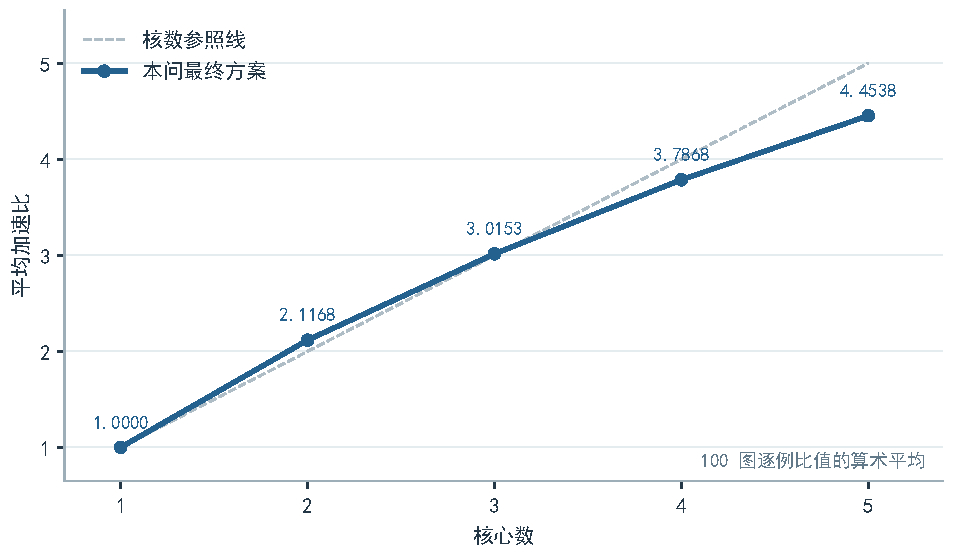
\includegraphics[width=.90\textwidth]{../求解/问题二/图片/q2_mean.pdf}
\caption{第二问各核数平均加速比}\label{fig:q2_mean}
\end{figure}

五核逐例加速比介于 $1.9919$ 和 $8.7768$，有 1 图低于 2，22 图高于 5。相对于原始整图单核参考，五核方案还调整了划分和核内顺序，搬运与自动换出也可能随之变化；因此这里的加速比可以超过五倍。五核周期的全局下界与当前结果所给相对差距上界，逐图平均为 $0.2462$；其中 6 图的界在 $1\%$ 以内。其余图的下界与可行周期之间仍有较宽区间。

图~\ref{fig:q2_distribution} 将同一批图的第一、二问五核加速比放在共同尺度上，并保留逐图点。第二问的分布整体向较高加速比移动，但仍有长尾与个别反例。为直接比较同一算例在两问中的执行周期，定义
\begin{equation}
 R_i=\frac{C_{i,1,5}}{C_{i,2,5}},\qquad i=1,\ldots,100.
 \label{eq:q2_pairratio}
\end{equation}
由于两问都以相同的 $T_{i,0}$ 定义加速比，$R_i$ 亦等于同图第二问加速比除以第一问加速比。100 图中 $R_i>1$ 有 89 图，$R_i=1$ 有 9 图，$R_i<1$ 有 2 图；比值均值 $1.1728$、中位数 $1.0913$。这组独立寻优结果表明，核心级 Task 下取得的最终方案在多数算例上更快。
\begin{figure}[htbp]\centering
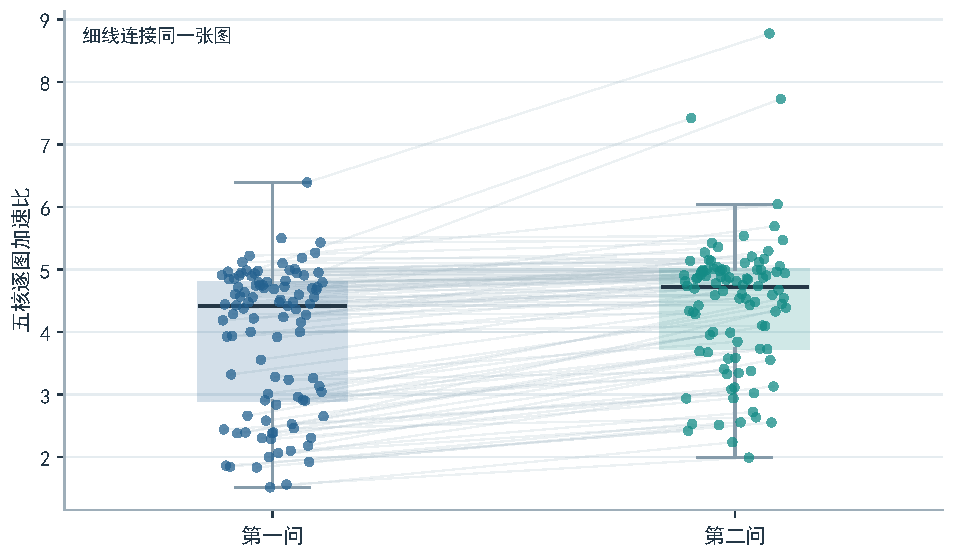
\includegraphics[width=.94\textwidth]{../求解/问题二/图片/q2_distribution.pdf}
\caption{五核逐图第一、二问加速比分布}\label{fig:q2_distribution}
\end{figure}

\subsubsection{COPY 量、驻留压力与反例}
第二问五核额外 COPY 字节的均值为 $8094619.10$ B，中位数为 $1310458$ B，均低于第一问的 $14585335.66$ B 和 $1990466$ B。逐图比较中，第二问有50个算例的额外COPY更少、12个相同、38个更多。图~\ref{fig:q2_copy} 按第二问减第一问的五核额外COPY字节差从小到大排列100个算例，依次分成四组，每组25个；纵轴为各问周期与本算例单核参考周期之比，每条线连接同一算例。COPY增加仍可能伴随周期缩短，因为方案可换取更早的跨核释放或更多计算重叠；COPY减少亦可能被更长的驻留区间和共享带宽争用抵消。
\begin{figure}[htbp]\centering
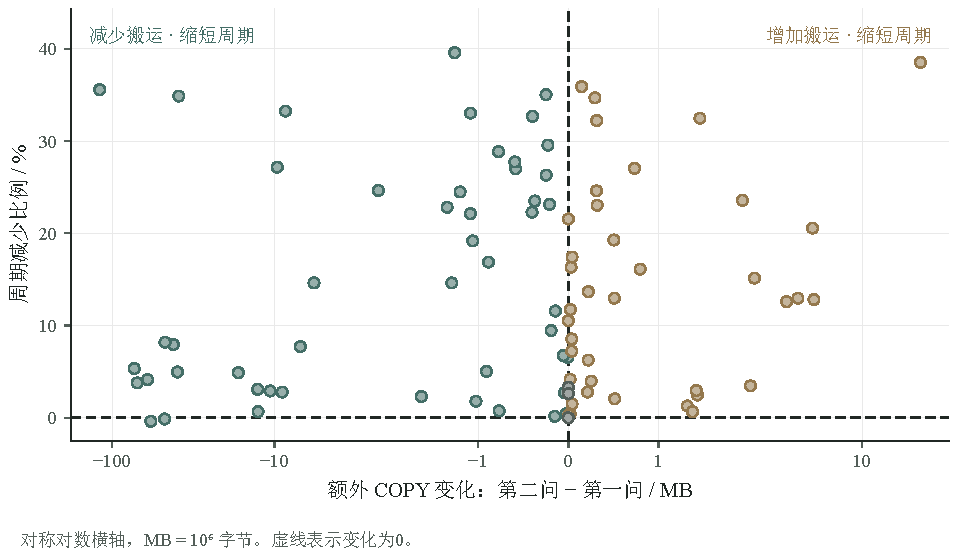
\includegraphics[width=.94\textwidth]{../求解/问题二/图片/q2_copy.pdf}
\caption{按COPY变化量分组的五核周期配对}\label{fig:q2_copy}
\end{figure}

边界搬运减少的同时，还需考察自动换出的变化。第一问五核有 88 图无自动换出，第二问为 74 图；第二问五核自动换出新增 COPY 字节的逐图均值为 $2645062.08$ B，高于第一问的 $206080.96$ B。同核驻留期延长可能增加容量压力，本组结果也记录到了更高的平均换出字节量。各算例的具体瓶颈仍需结合其执行轨迹定位。第二问周期略长的两个算例分别为算例072和算例079，其第一、二问五核周期为 $4775553/4781658$ 与 $5985137/6007992$；二者的第二问额外 COPY 字节反而都更少。这两个算例表明，额外COPY减少与周期缩短并不总是同步；关键路径、Pipe排队、活跃缓冲和DDR发射时机提供了进一步分析的方向。

\subsubsection{候选来源的调用与改善}
图~\ref{fig:q2_sources} 汇总第二问实际候选来源的调用和周期改善记录。结构来源完成评价 $15656$ 次，其中 $740$ 次带来周期改善；基础来源为 $8589$ 次及 $443$ 次，驻留来源为 $8819$ 次及 $353$ 次。三类来源均在联合搜索中取得过周期改善。它们相继更新同一个当前方案，调用机会随图结构、近期收益和剩余预算变化；这里统计的是联合运行表现，各来源的独立贡献有待控制来源的对照实验评估。
\begin{figure}[H]\centering
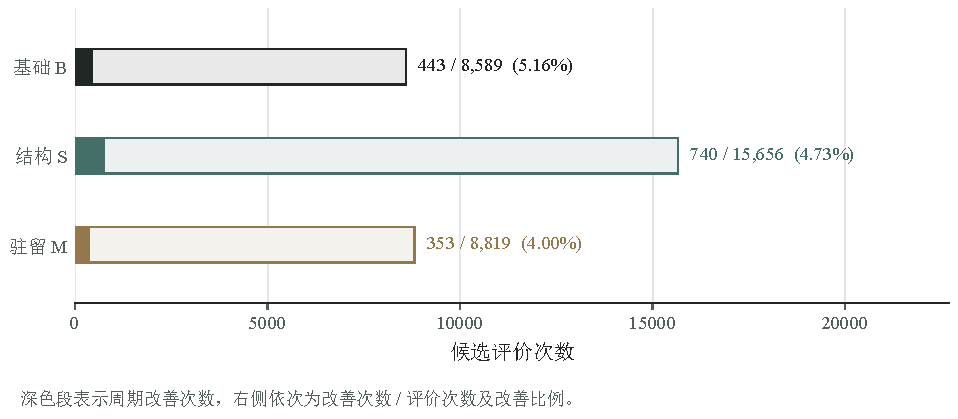
\includegraphics[width=.94\textwidth]{../求解/问题二/图片/q2_sources.pdf}
\caption{第二问候选来源的调用与周期改善记录}\label{fig:q2_sources}
\end{figure}

综合逐图周期、COPY 量和存储记录，第二问的主要机会来自同核跨子图复用与更细的跨核释放，但两者同时改变并行性和片上驻留压力。下一问在本问核心级 Task 基础上加入共享只读缓存，需进一步把逻辑 COPY 请求量与实际 DDR 服务量区分。
